\chapter{Contextualização Tecnológica}



\section{A Empresa TecSus}
\par A Empresa TecSUS Tecnologias para a Sustentabilidade, é uma \emph{startup} de tecnologia da informação que atua no desenvolvimento de dispositivos, aplicativos e sistemas para transmissão e recepção de dados, controle de equipamentos remotos e gestão da informação, aplicados predominantemente nos setores de abastecimento de água, saneamento, geração e distribuição de eletricidade, distribuição de gás natural, e serviços municipais, embora as aplicações possam ter caráter mais abrangente. As tecnologias visam aprimorar o uso dos recursos naturais do planeta, contribuindo para a redução do desperdício (de água, energia, gás e tempo) e tornando a gestão destes recursos mais eficiente.


\section{A Coleta dos dados}
\par A Empresa TecSUS coleta informações para monitoramento de consumo de água. O serviço é oferecido tanto para residências como para estabelecimentos comerciais. Veja a ilustração do serviço prestado na figura \ref{techid}.
\begin{figure}[ht]
	\caption{\textbf{TecHydro Monitoramento e Controle remoto de hidrômetros}}
	\centering
		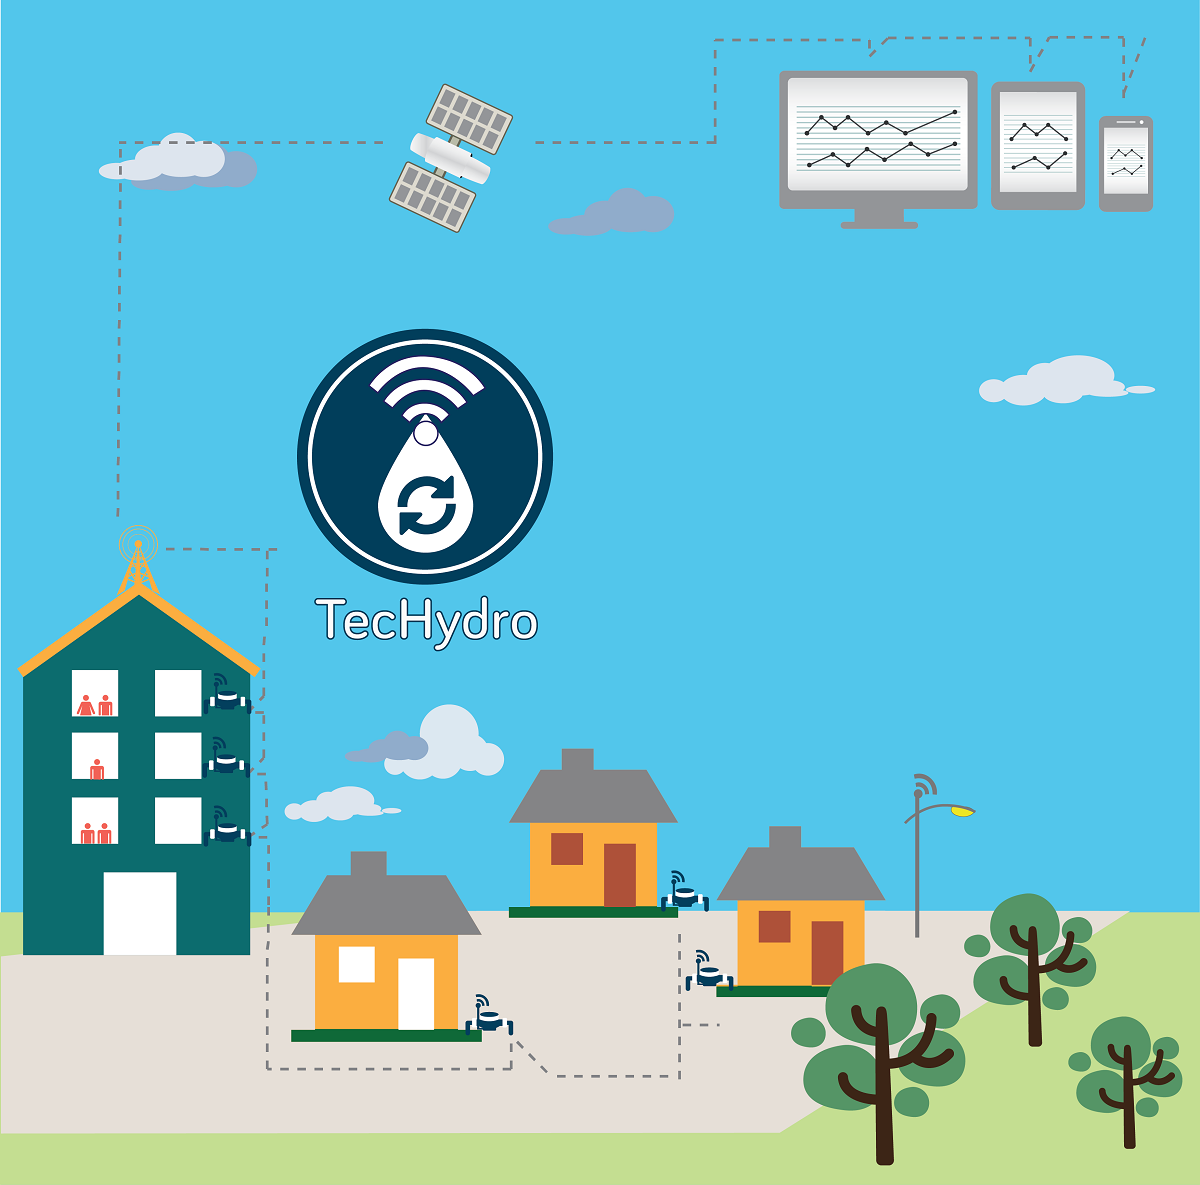
\includegraphics[scale=0.3]{figuras/TecHydro}
	\fonte{TecSUS(2018).}
	\label{techid}
\end{figure}

\par Os dados são coletados diretamente dos hidrômetros, por uma placa eletrônica da TecSus. Esses dados são transmitidos em uma rede \emph{mesh} local, até chegar a um concentrador de dados que fica no cliente.
\par O concentrador de dados tem acesso à \emph{internet} e enviam esses dados para a nuvem através de MQTT \emph{(Message Queuing Telemetry Transport)}, os dados quando chegam à nuvem são processados e armazenados no banco de dados.


\section{Dados e Informação}

\par Com é explicado em  \cite{Elias}, os dados não tem  significado relevante não conduz uma compreensão com exatidão, os dados podem ser com exemplo uma \emph{string} ou um caractere numérico ou alfabético ou simbolos e caracters especiais.
\par E a informação é a ordenação e a organização dos dados de forma que transmita um significado ou uma compreensão dentro de um determinado contexto. O conjunto ou consolidação dos dados de forma a fundamentar o conhecimento.
\par Quanto mais distanciamos dos dados maior é a abstração, como pode ser observado na figura \ref{abst}
\begin{figure}[ht]
	\caption{\textbf{Abstração}}
	\centering
		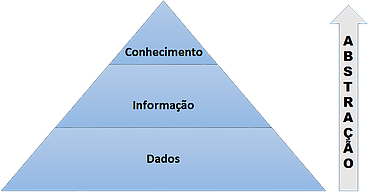
\includegraphics[width=\textwidth,height=\textheight, keepaspectratio]{figuras/abstracao}
		\label{abst}
	\fonte{\cite{Elias}}
\end{figure}


\section{\emph{Data Mining} (Mineração de Dados) e KDD}
%\label{minerdados}

\subsection{\emph{Data Mining} (Mineração de Dados)}

\par A mineração de dados geralmente faz parte de uma maior inteligência de negócios ou gerenciamento de conhecimento
iniciativa conforme é explicado em \cite{dig2004privacy}. Como os governos estaduais são organizações complexas que coletam e processam grandes quantidades de informações, a mineração de dados pode ajudar a fornecer valor ao governo estadual operações e contribuintes através da extração de informações úteis das montanhas de
dados. Além disso, a mineração de dados pode ser preditiva e descobrir padrões ocultos que
pode estrategicamente usar para reduzir custos, aumentar as oportunidades de expansão de negócios, e detectar fraudes, desperdícios e abusos que drenam os dólares dos contribuintes.
\par O objetivo da mineração de dados é identificar padrões para fazer previsões a partir de
informações contidas em bancos de dados. Ele permite que o usuário seja proativo na identificação e predizendo tendências com essa informação. Usos comuns de mineração de dados no governo incluem descoberta de conhecimento, detecção de fraudes, análise de pesquisa, suporte à decisão e personalização do site. Os usos mais comuns do governo federal de mineração de dados
identificados pelo GAO(U.S. General Accounting Office (GAO)) incluem:
\begin{itemize}
\item Melhorar o serviço ou desempenho
\item Detectar fraude, desperdício e abuso
\item Analisar informações científicas e de pesquisa
\item Gestão de recursos humanos
\item Detectar atividades ou padrões criminosos
\item Analisar inteligência e detectar atividades terroristas
\end{itemize}

\subsection{KDD \emph{(Knowledge Discovery in Databases)}}

\par O processo capaz de descobrir conhecimento (informação) em banco de dados chama-se KDD \emph{(Knowledge Discovery in Databases)}, este processo foi proposto em 1989 por\cite{fayyad1996data}, para referir-se as etapas que produzem conhecimento a partir de dados. Dentro deste processo a etapa de mineração de dados é a fase que transforma dados em informação.
\par Definida como o processo de descoberta de padrões nos dados por  \cite{fayyad1996data}, com o objetivo de explicar a informação e a realizar predições a partir da mesma. A prática de mineração de dados tem como objetivo produzir informação na forma de fatos ou padrões, também chamados conhecimento adquirido segundo \cite{fayyad1996data}. Este conhecimento para ser corretamente interpretado e útil, deve ser apresentado de forma a atingir tal propósito, apresentando assim o que foi aprendido para poder realizar reflexões a partir do mesmo. Pode se observar os processos do KDD com mais clareza na figura \ref{kdd} .
\begin{figure}[h]
	\caption{\textbf{Etapas do processo KDD}}
	\centering
		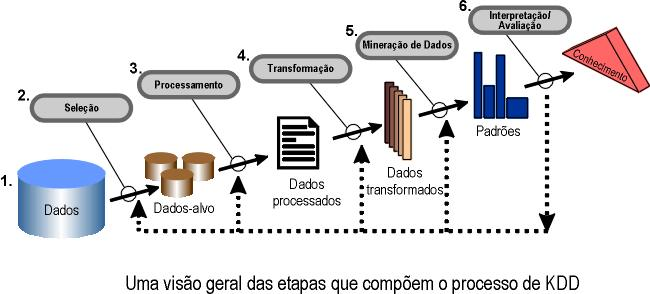
\includegraphics[width=\textwidth,height=\textheight, keepaspectratio]{figuras/processo de kdd.jpg}
		\label{kdd}
	\fonte{\cite{fayyad1996data}}
\end{figure}
\par O processo inicia-se com a obtenção dos dados. Depois etapa de seleção, é onde serão decididos quais os conjuntos de dados que serão relevantes para que sejam obtidos resultados com informações uteis. Na etapa de processamento acontece à limpeza dos dados e seleção de atributos. Nesta etapa informações ausentes errôneas ou inconsistentes nas bases de dados devem ser corrigidas de forma a não comprometer a qualidade dos modelos de conhecimento a serem extraídos ao final do processo de KDD. A etapa de transformação dos dados analisa os dados obtidos da etapa anterior e os reorganiza de uma forma especifica para que possam ser interpretados na etapa seguinte. Na etapa de mineração dos dados é onde tudo acontece, os dados depois de transformados serão lidos e interpretados. A mineração faz com que meros dados sejam transformados em informações, tais informações são indicadas através de força bruta, ou seja, lendo regra por regra e as interpretando. Na última etapa a de interpretação de resultados é onde as regras indicadas pelo processo anterior serão interpretadas e avaliadas. 
\section{Distância Euclidiana}
%\label{distan}
\par A distância euclidiana é uma medida de Dissimilaridade, é um conceito matemático que representa a menor distância existente entre dois pontos na Geometria Euclidiana. Esta geometria foi construída pelo matemático grego Euclides. Segundo  \cite{regazzi2002analise}, “embora a distância euclidiana seja uma medida de dissimilaridade, às vezes ela é referida como uma medida de semelhança, pois quanto maior seu valor, menos parecidos são os indivíduos ou unidades amostrais”, quanto menor o valor observado mais parecido serão os objetos ou nesse caso os pontos da série temporal. A Distância Euclidiana só pode ser medida em séries do mesmo tamanho, consistindo no cálculo da distância entre os pares de pontos das duas sequencias.
\par O calculo  tem complexidade O(n), mas pode ser acelerado. Quando ela é utilizada como sub-rotina em algoritmos de mineração como o de classificação, por exemplo, o interesse pode estar em conhecer a verdadeira distância entre séries.
\par De acordo com \cite{manly2016multivariate}, “a distância euclidiana, quando for estimada a partir das variáveis originais, apresenta a inconveniência de ser influenciada pela escala, de medida pelo número de variáveis e pela correlação existente entre as mesmas”. Para contornar as escalas, faz-se a padronização das variáveis em estudo, para que possuam a variância igual à unidade.
\par Distância entre duas instâncias $P_i$ e $P_j$ definida como:
\begin{figure}[ht]
\caption{\textbf{Distância Euclidiana}}
\centering

    \newlength\dlf
    \newcommand\alignedbox[2]{
      % #1 = before alignment
      % #2 = after alignment
      &
      \begingroup
      \settowidth\dlf{$\displaystyle #1$}
      \addtolength\dlf{\fboxsep+\fboxrule}
      \hspace{-\dlf}
      \fcolorbox{black}{gray!30}{$\displaystyle #1 #2$}
      \endgroup
    }

    \begin{align}\
        \alignedbox{}{D=\sqrt{ \sum\limits_{k=1}^n (P_{ik}-P_{jk})^2}}
    \end{align}
       \label{distancia_euclidiana}
       \fonte{\cite{manly2016multivariate}}
    \end{figure}

\par $P_{ik}$ e $P_{jk}$ para K = 1..., n. São os n que descrevem as instâncias $p_i$ e $p_j$, respectivamente.
\par A distância euclidiana é, sem dúvida, a medida de distância mais utilizada para a análise de agrupamentos e para análise de séries temporal. Considerando o caso mais simples, no qual existem n indivíduos, onde cada um dos quais possuem valores para p variáveis, a distância euclidiana entre eles é obtida mediante o teorema de Pitágoras, para um espaço multidimensional.
\par Explicando a formula, é a raiz quadrada da soma dos resultados da diferença entre os pontos elevados ao quadrado, pode ser observada na figura \ref{distancia_euclidiana}. 

\section{Linguagem Python, e suas bibliotecas e ferramentas}

\par Para ter mais eficiência na análise de dados foi utilizada a linguagem \emph{Python} e também utiliza-se algumas bibliotecas destinadas para análise de dados e cálculos específicos.
\par O \emph{ \cite{python}} é uma linguagem de programação criada por \emph{Guido Van Rossum} em 1991,  é a linguagem ideal para aplicações científica sendo uma linguagem expressiva, em que é fácil traduzir o raciocínio em um algoritmo e tem sido ótimo para dados e preparação, e para análise e modelagem de dados.
\par A \cite{pandas}  é uma biblioteca \emph{open source}, licenciada pelo BSD, que por sua vez é uma licença de código aberto inicialmente utilizada nos sistemas operacionais do tipo \emph{Berkeley Software Distribution}, que fornece estruturas de dados de alto desempenho e fáceis de usar e ferramentas de análise de dados para a linguagem de programação \emph{Python}. A biblioteca ajuda a preencher essa lacuna, permitindo que você execute todo o seu fluxo de trabalho de análise de dados em Python sem precisar alternar para um idioma mais específico do domínio, como Linguagem R. Combinado com o excelente \emph{kit} de ferramentas \emph{IPython} e outras bibliotecas, o ambiente para análise de dados no Python se destaca no desempenho, produtividade e capacidade de colaboração. 
\par A biblioteca \cite{numpy} é descrita  como o pacote básico da linguagem \emph{Python} que permite trabalhar com arranjos, vetores e matrizes de N dimensões, de uma forma comparável e com uma sintaxe semelhante ao \emph{software} proprietário \emph{Matlab}, mas com muito mais eficiência, e com toda a expressividade da linguagem.
\par A biblioteca \emph{ \cite{matplotlib}}, é uma biblioteca de plotagem 2D em \emph{Python} que produz números de qualidade de publicação em uma variedade de formatos impressos e ambientes interativos entre plataformas. O \emph{Matplotlib} pode ser usado em \emph{scripts Python}, nos \emph{shells} do \emph{Python} e do \emph{IPython}, no \emph{Notebook Jupyter}, nos servidores de aplicativos da \emph{Web} e em quatro \emph{kits} de ferramentas de interface gráfica do usuário.
\par  E   para fazer a integração da linguagem \emph{python} com as bibliotecas, pode-se utilizar vários compiladores, IDE (\emph{Integrated Development Environment})  que   \'e o  Ambiente de Desenvolvimento Integrado,  \emph{Pycharm}, \emph{Visual Studio}, \emph{Notepad++} e o \emph{Jupyter Notebook}, onde o mesmo foi utilizado para a análise dos dados e plotagem dos gráficos. 
\par O \emph{ \cite{jupyter}}, a explicação que é um aplicativo da \emph{Web} de código aberto que permite criar e compartilhar documentos que contêm código ativo, equações, visualizações e texto narrativo. Os usos incluem: limpeza e transformação de dados, simulação numérica, modelagem estatística, visualização de dados, aprendizado de máquina e muito mais. Nascido do Projeto \emph{IPython} em 2014, à medida que evoluiu para suportar ciência de dados interativa e computação científica em todas as linguagens de programação.   